\chapter{Demodulation Algorithms}
After discussing the different demodulation techniques it is time to have some more discussion of software based demodulation techniques, specifically. However, before talking about the algorithms for doing the FSK demodulation it is worth specifying what type of FSK Bell 202 is. There are two features that are relevant for taking into consideration when demodulating the signal. First, is that it is asynchronous meaning that there is no separate clocking signal and it is embedded within the data signal. If it were synchronous there would be two different signals coming into the demodulator which would be the data carrier signal and a clocking signal. The second characteristic is that the FSK is coherent or continuous. This means that there is a continuous signal at bit boundaries and there are no jumps as the signal changes from one frequency to another. Below there are two figures that show examples of both non-coherent transitions and coherent transitions. It might be noticed that some of the figures used in the discussion previously also exhibited the coherent characteristic. The next few sections are general approaches that can be used for any FSK demodulation. In addition to describing each generally some specific details of APRS Bell 202 demodulation. 
\begin{figure}
  \centering
	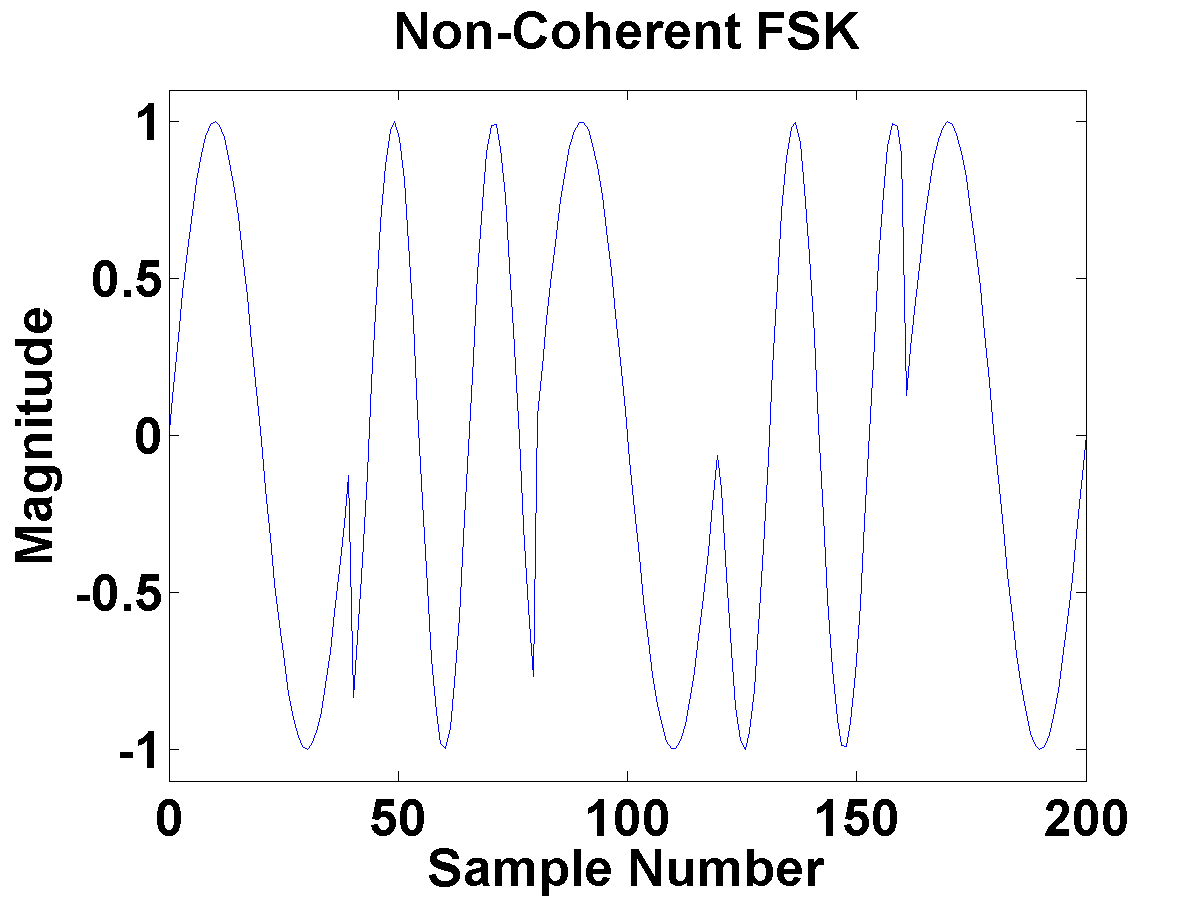
\includegraphics[width=0.75\linewidth]{images/NonCoherentFSK.png} 
	\caption{Example of a non-coherent 1200Hz / 2200Hz FSK signal.}
\end{figure}
\begin{figure}
  \centering
	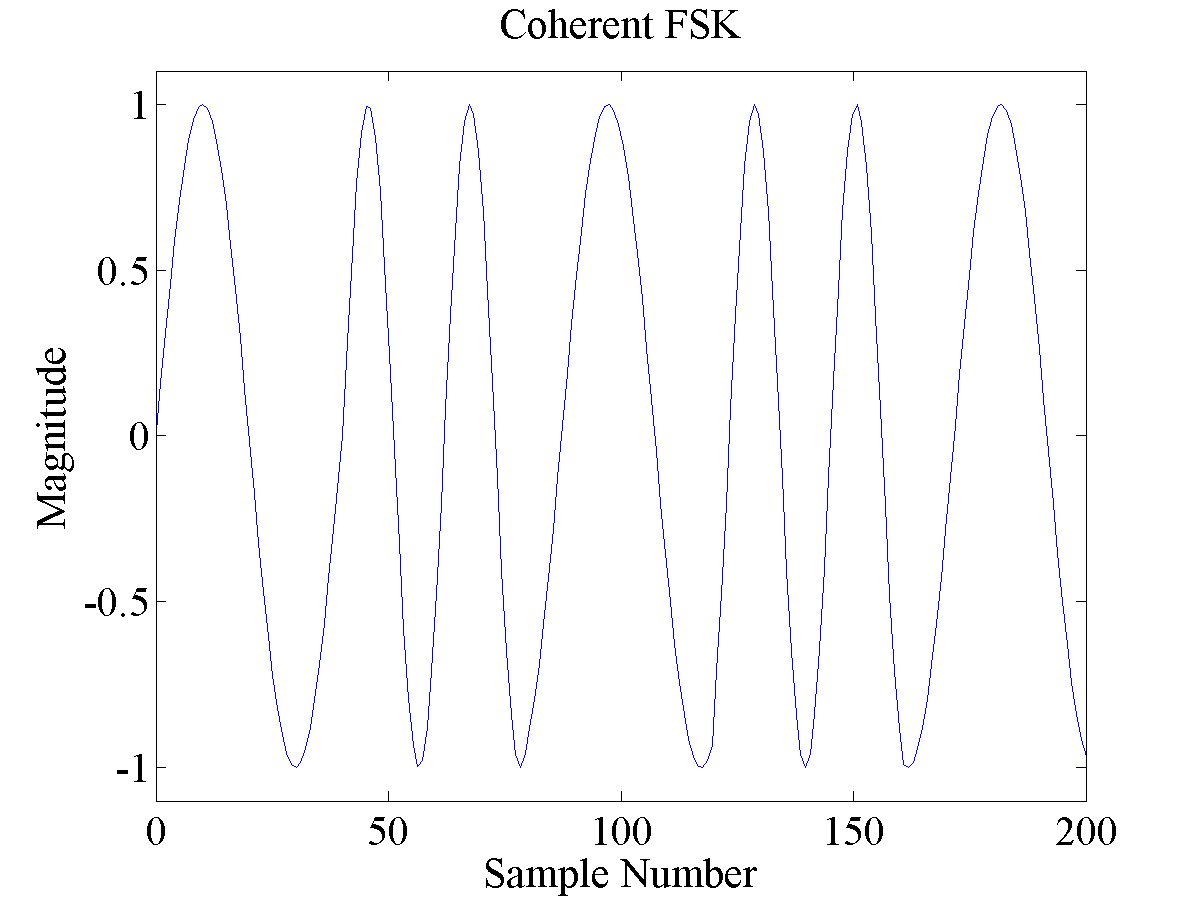
\includegraphics[width=0.75\linewidth]{images/CoherentFSK.png} 
	\caption{Example of a non-coherent 1200Hz / 2200Hz FSK signal.}
\end{figure}

\section{Zero Crossing}
Using zero crossings to determine the frequency of the FSK signal is one of the the easiest algorithms from a software implementation perspective. The idea is that based off of the time elapsed between zero crossings of the signal the period of the waveform can be measured. Once the period has been calculated the frequency can then be easily calculated using the inverse relationship between period and frequency, \textit{f} = 1 /T where \textit{f} is the frequency and T is the period. It is worth noting and keeping in mind that two consecutive zero crossings are only half of the period since there are a total of three zero crossings in one period.

\section{Correlation}
Another method that can be used for demodulation of FSK is correlation with the underlying FSK signals. For APRS this is done by synthesizing a 1200Hz tone and a 2200Hz tone and then comparing the input signal to each of these. Which ever one of the synthesized signals the input signal is more similar to - has more correlation with - the input signal must be the frequency that is present at that point in time in the data carrying signal. 

\section{Discrete Fourier Transform}
A discrete Fourier Transform is one implementation of Fourier Transform that is used on discrete samples similar to what is present in a digital audio file. Once a Fourier transform has been applied on a signal the output is a relative power versus frequency. With this data which ever frequency, either 1200Hz or 2200Hz, is more prominent is which symbol must be present in the bit period. 

\section{Phase Lock Loop}
A phase lock loop (PLL) is exactly what the name implied. It is a loop that stays locked onto the phase of the input signal. This is done by taking input signal detecting the phase and then producing an output the corresponds with the phase. The output is fed back in with the input so that any differences between the input and output of the phase lock loop can be reconciled to have a phase exactly in phase with the input. The convenient thing about monitoring the phase of the signal so closely and being able to stay locked onto it is that the frequency must also be known. Extracting this frequency information from the PLL can hence be used for FSK demodulation.

\section{Advantages of Using the Derivative of the Original Signal}
One thing considered while trying to demodulate the Bell 202 signals was the implications of using the derivative of the signal for decoding as opposed to the actual signal. One advantage that was seen through using this approach is that for cases where there is a DC offset of the signal, the derivative would remove this and re-center the signal about zero. A consequence of using the derivative of a sine wave signal is that the result will be 90 degrees out of phase. It was decided that this would not be a problem since the whole signal would be 90 shifted by this amount and the timing is done on the fly once the signal is received anyways. However, there were some other things about using the derivative that were not considered until later. One thing is that in addition to to helping the DC offset it also helps signals that were de-emphasized by not pre-emphasized. In signals where this is the case the 2200Hz tones will be lower in the original signal, but since they have a steeper slope this ends up helping to normalize these differences in the resulting derivative. Although the derivative helps with this, it will hurt if the opposite is the case (preemphasized but not deemphasized) only worsening the problem.
\begin{figure}
  \centering
	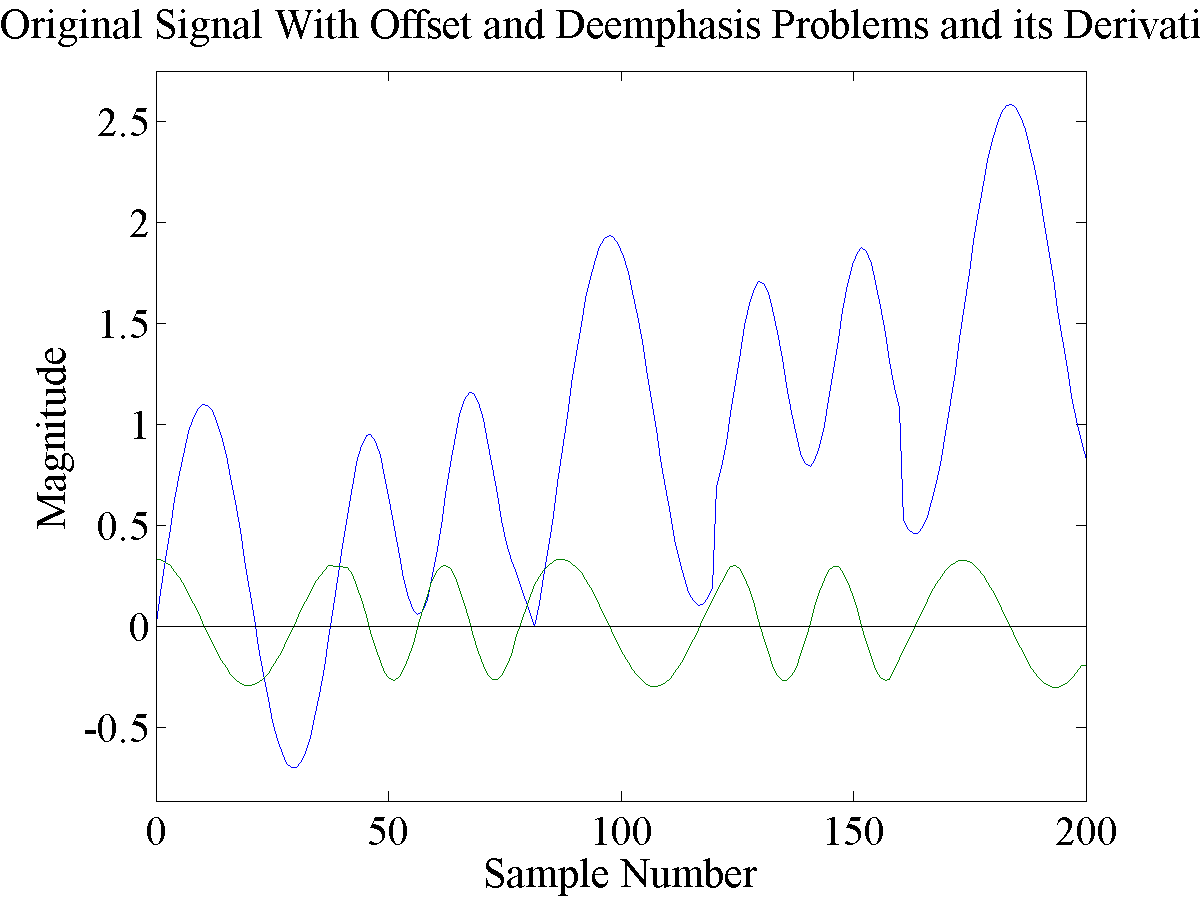
\includegraphics[width=0.75\linewidth]{images/OriginalSignalWithOffsetandDeemphasisProblemsanditsDerivative.png} 
	\caption{Example of a signal that has both a DC offset and a deemphasis problem and its corresponding derivative.}
\end{figure}
